\documentclass[border=10pt]{standalone}
\usepackage{tikz,amsmath}
\usetikzlibrary{arrows.meta}

\definecolor{hidFill}{RGB}{199,203,243}
\definecolor{hidLine}{RGB}{52,58,143}
\definecolor{inFill}{RGB}{183,224,177}
\definecolor{inLine}{RGB}{32,102,32}
\definecolor{outFill}{RGB}{243,199,199}
\definecolor{outLine}{RGB}{143,52,52}

\begin{document}
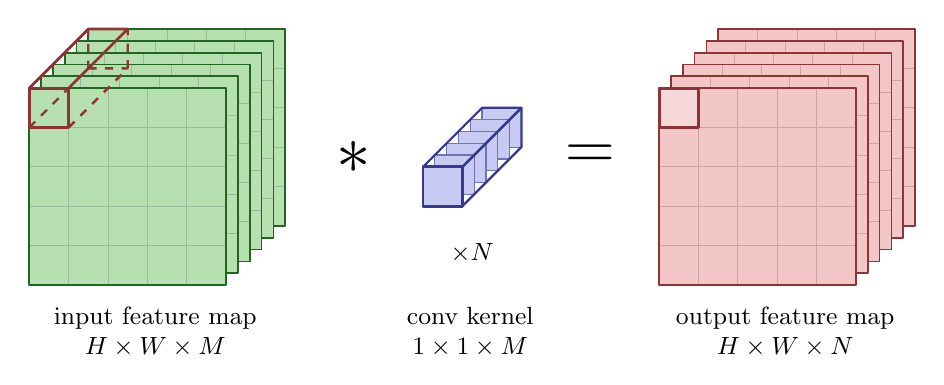
\begin{tikzpicture}[
    font=\small, line join=round,
    every node/.style={inner sep=0pt, outer sep=0pt, align=center}
  ]

  % 通用带网格平板宏: #1=x, #2=y, #3=格子数, #4=格长, #5=颜色前缀
  \newcommand{\gridplate}[5]{%
    \fill[#5Fill] (#1,#2) rectangle (#1+#3*#4, #2+#3*#4);
    \draw[step=#4, #5Line!45, line width=.35pt, shift={(#1,#2)}] (0,0) grid (#3*#4, #3*#4);
    \draw[#5Line, line width=.6pt] (#1,#2) rectangle (#1+#3*#4, #2+#3*#4);
  }

  % 1. 输入特征图：H x W x M (从后向前绘制 5 -> 0)
  \foreach \i in {5,4,...,0}{%
    \gridplate{\i*.15}{\i*.15}{5}{.5}{in}
  }

  % 1x1 跨通道感受野透空线框
  \draw[outLine, dashed, line width=.85pt] 
    (0.5, 2.0) -- (1.25, 2.75)
    (1.25, 2.75) -- (1.25, 3.25)
    (0.75, 2.75) -- (1.25, 2.75)
    (0, 2.0) -- (0.75, 2.75) -- (0.75, 3.25);

  \draw[outLine, line width=1.0pt] 
    (0, 2.5) -- (0.75, 3.25) -- (1.25, 3.25)
    (0.5, 2.5) -- (1.25, 3.25);

  \draw[outLine, line width=1.15pt] (0, 2.0) rectangle (0.5, 2.5);

  \node at (1.6, -0.6) {input feature map\\$H\times W\times M$};

  % 2. 卷积运算符
  \node[font=\Huge] at (4.125, 1.625) {$\ast$};

  % 3. 卷积核：1 x 1 x M (居中对齐至 y=1.625)
  \foreach \i in {5,4,...,0}{%
    \fill[hidFill] (5.0+\i*.15, 1.0+\i*.15) rectangle (5.0+\i*.15+.5, 1.0+\i*.15+.5);
    \draw[hidLine!70, line width=.4pt] (5.0+\i*.15, 1.0+\i*.15) rectangle (5.0+\i*.15+.5, 1.0+\i*.15+.5);
  }
  \draw[hidLine, line width=.8pt] (5.0, 1.5) -- (5.75, 2.25) -- (6.25, 2.25) -- (5.5, 1.5) -- cycle;
  \draw[hidLine, line width=.8pt] (5.5, 1.5) -- (6.25, 2.25) -- (6.25, 1.75) -- (5.5, 1.0) -- cycle;
  \draw[hidLine, line width=1pt] (5.0, 1.0) rectangle (5.5, 1.5);

  \node[font=\small] at (5.625, 0.4) {$\times N$};
  \node at (5.6, -0.6) {conv kernel\\$1\times 1\times M$};

  % 4. 等号
  \node[font=\Huge] at (7.125, 1.625) {$=$};

  % 5. 输出特征图：H x W x N (6 层，居中对齐至 y=1.625)
  \foreach \i in {5,4,...,0}{%
    \gridplate{8.0+\i*.15}{\i*.15}{5}{.5}{out}
  }
  \fill[outFill!70] (8.0, 2.0) rectangle (8.5, 2.5);
  \draw[outLine, line width=1.1pt] (8.0, 2.0) rectangle (8.5, 2.5);

  \node at (9.6, -0.6) {output feature map\\$H\times W\times N$};

\end{tikzpicture}
\end{document}